\documentclass{article}
\usepackage{tikz}
\usepackage{circuitikz}
\usepackage{booktabs}
\usepackage{amsmath}

\title{Apuntes de L\'{o}gica Digital}
\date{2023-05-08}
\author{Daniel Araya Rom\'{a}n}

\begin{document}
\maketitle
\newpage

\section*{1. Sistemas Binarios}

\paragraph*{}
\normalsize

\subsection*{1.1 Sistemas Digitales}

En los sistemas digitales electr\'{o}nicos actuales,
las se\~{n}ales emplean s\'{o}lo dos valores discretos
$\rightarrow binarios$. Un d\'{i}gito binario, llamado
\textbf{bit}, que puede tomar los valores 0 y 1.
Un sistema digital es una interconexi\'{o}n de m\'{o}dulos
digitales. Para entender como funciona cada m\'{o}dulo digital,
se necesiatan conocimientos b\'{a}sicos de circuitos digitales
y de su funci\'{o}n l\'{o}gica.

Un lenguaje importante para el dise\~{n}o digital es el \textbf{(HDL,
Hardware Description Language)}. Sirve para simular sistemas digitales
y verificar su funcionamiento antes de crearlos en hardware.
\medskip

\begin{center}
    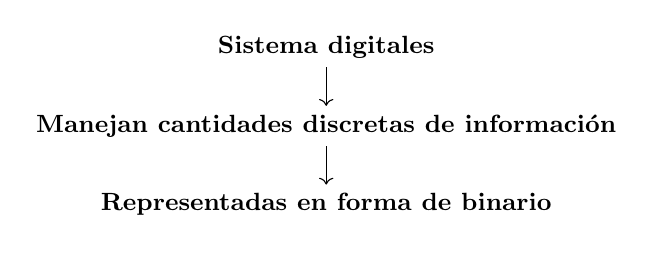
\begin{tikzpicture} 
        \small
        \node (a) at (0,0) {\textbf{Sistema digitales}};
        \node (b) at (0,-1) {\textbf{Manejan cantidades discretas de informaci\'{o}n}};
        \node (c) at (0,-2) {\textbf{Representadas en forma de binario}};
        \draw[->] (a) -- (b);
        \draw[->] (b) -- (c);
    \end{tikzpicture}
\end{center}
\medskip

\subsection*{1.2 N\'{u}meros Binarios}

\paragraph*{}
\normalsize

El n\'{u}mero decimal 7392, contiene potencias de 10 que est\'{a}n
impl\'{i}citas en la posici\'{o}n de los coeficientes, e.g:
\medskip

\begin{center}
    $7 \times 10^3 + 3 \times 10^2 + 9 \times 10^1 + 2 \times 10^0$
\end{center}

Un n\'{u}mero con punto decimal se representa con una serie de 
coeficientes, as\'{i}:

\begin{center}
    \large
    $a_5a_4a_3a_2a_1a_0 \cdot a_{-1}a_{-2}a_{-3}$
\end{center}

los coeficientes $a_j$ son cualesquiera de los 10 d\'{i}gitos (0...9);
el valor del sub\'{i}ndice $j$ indica la posici\'{o}n, y la potencia de
10 que se deber\'{a} multplicar ese coeficiente. De modo que:

\begin{center}
    $10^5a_5 + 10^4a_4 + 10^3a_3 + 10^2a_2 + 10^1a_1 + 10^0a_0
     + 10^-1a_{-1} + 10^-2a_{-2} + 10^-3a_{-3}$
\end{center}

El sistema binario es distinto al decimal, sus coeficientes solo pueden
tener 2 valores, 0 o 1. Cada coeficiente $a_j$ se multiplica por $2^j$.
11010.11 es 26.75 en decimal, porque:

\begin{center}
    $1 \times 2^4 + 1 \times 2^3 + 0 \times 2^2 + 1 \times 2^1 + 0 \times 2^0
     + 1 \times 2^{-1} + 1 \times 2^{-2} = 26.75$
\end{center}

En general, un n\'{u}mero expresado en un sistema de base \textbf{r} consiste
en coeficientes que se multiplican por potencias de \textbf{r}:

\begin{center}
    $a_n \cdot r^n + a_{n-1} \cdot r^{n-1} +...+ a_2 \cdot r^2 + a_1 \cdot r 
     + a_0 + a_{-1} \cdot r^{-1} + a_{-2} \cdot r^{-2} +...+ a_{-m} \cdot r^{-m}$
\end{center}

\subsection*{1.4 N\'{u}meros Octales y Hexadecimales}

Las conversiones entre binario, octal y hexadecimal son importantes en las 
computadoras digitales. Puesto que $2^3 = 8$ y $2^4 = 16$, cada d\'{i}gito
octal corresponde a \textbf{tres} d\'{i}gitos binarios, y cada d\'{i}gito
hexadecimal corresponde a \textbf{cuatro} d\'{i}gitos binarios.

$Binario \rightarrow octal$: agrupando los d\'{i}gitos binarios de 3 en 3,
de derecha a izquierda, y reemplazando cada grupo por su equivalente octal.
\begin{center}
    \large
    $(10\,110\,001\,101\,011 \cdot 111\,100\,000\,110)_2 = (26153.7406)_8$
\end{center}

$Binario \rightarrow hexadecimal$: agrupando los d\'{i}gitos binarios de 4 en 4,
de derecha a izquierda, y reemplazando cada grupo por su equivalente hexadecimal.
\begin{center}
    \large
    $(10\,1100\,0110\,1011 \cdot 1111\,0010)_2 = (2C6B.F2)_{16}$
\end{center}

Cuando se habla de binario es m\'{a}s deseable expresarlo en t\'{e}rminos de
n\'{u}meros octales o hexadecimales, porque son m\'{a}s compactos y f\'{a}ciles
de leer. As\'{i} $(111\,111\,111\,111)_2$ este n\'{u}mero en binario de 12 bits,
se puede escribir como $(7777)_8$ en octal o $(FFF)_{16}$ en hexadecimal.

\medskip

\begin{table}[h]
    \centering
    \begin{tabular}{cccc}
        \toprule
        Decimal & Binary & Octal & Hexadecimal \\
        (base 10) & (base 2) & (base 8) & (base 16) \\
        \midrule
        0 & 0000 & 00 & 0 \\
        1 & 0001 & 01 & 1 \\
        2 & 0010 & 02 & 2 \\
        3 & 0011 & 03 & 3 \\
        4 & 0100 & 04 & 4 \\
        5 & 0101 & 05 & 5 \\
        6 & 0110 & 06 & 6 \\
        7 & 0111 & 07 & 7 \\
        8 & 1000 & 10 & 8 \\
        9 & 1001 & 11 & 9 \\
        10 & 1010 & 12 & A \\
        11 & 1011 & 13 & B \\
        12 & 1100 & 14 & C \\
        13 & 1101 & 15 & D \\
        14 & 1110 & 16 & E \\
        15 & 1111 & 17 & F \\
        \bottomrule
    \end{tabular}
    \caption{N\'{u}meros en diferentes bases.}
    \label{tab:numbers}
\end{table}

\newpage
\subsection*{1.5 Complementos}

En las computadoras digitales se usan complementos para simplificar la
operaci\'{o}n de resta y para efectuar manipulaciones l\'{o}gicas. Existen
dos tipos de complementos para cada sistema de base $r$: el 
\textit{complemento a la base} y el \textit{complemento a la base disminuida.}
El primero se denomina complemento a $r$, mientras que el segundo es el complemento
a $(r - 1)$. Si se sustiyue el valor de la base $r$ en los nombres obtenemos que los
dos tipos son el complemento a 2 y el complemento a 1. 

\subsubsection*{1.5.1 Complemento a la base}
El complemento a $r$ de un n\'{u}mero $N$ de $n$ d\'{i}gitos en base $r$ se define
como: 
\begin{center}
    $r^n - N$, para $N \neq 0$, y 0 para $N = 0$. 
\end{center}
Por ejemplo, el complemento a 10 de 1234 es $10^4 - 1234 = 8766$.
De forma similar, el complemento a dos se forma dejando como están todos los
ceros menos significativos y el primer uno, y sustituyendo los unos por ceros y
los ceros por unos en las demás posiciones a la izquierda.
\begin{center}
    El complemento a dos de 1101100 es 0010100. \\
    El complemento a dos de 0110111 es 1001001.
\end{center}

\subsubsection*{1.5.2 Complemento a la base disminuida}
De igual manera, dado un n\'{u}mero $N$ en base $r$ que tiene $n$ d\'{i}gitos, el
complemento a $(r - 1)$ de $N$ se define como:
\begin{center}
    $(r^n - 1) - N$.
\end{center}

Con n\'{u}meros decimales, $r = 10$ y $r - 1 = 9$, as\'{i} el complemento
a nueve de $N$ es $(10^n - 1) - N$. El $10^n$ representado por $n$ \textit{nueves}.
Por ejemplo, si $n = 4$, tenemos $10^4 = 10,000$ y $10^4 - 1 = 9999$. El complemento
a nueve se consigue restando cada d\'{i}gito a nueve. $e.g$:
\begin{center}
    Complemento a nueve de 546700 es 999999 - 546700 = 453299. \\
    Complemento a nueve de 012398 es 999999 - 012398 = 987601. 
\end{center}

Ahora con n\'{u}meros binarios, $r = 2$ y $r - 1 = 1$, as\'{i} el complemento a uno
de $N$ es $(2^n - 1) - N$. En este caso $2^n$ se representa con un n\'{u}mero binario
que consite en un uno seguido de $n$ ceros.
\begin{center}
    $n = 4, \quad 2^4 = 10000_2$
\end{center}

Por otro lado $2^n -1$ es un n\'{u}mero binario representado por $n$ unos.
\begin{center}
    $n = 4, \quad 2^4 - 1 = 1111_2$
\end{center}

El complemento a uno se consigue invirtiendo cada d\'{i}gito. El restar d\'{i}gitos
binarios a uno podemos tener $1 - 1 = 0$ y $1 - 0 = 1$. Cambiando el bit de 0 a 1 o
de 1 a 0. $e.g$:
\begin{center}
    Complemento a uno de 101101 es 111111 - 101101 = 010010. \\
    Complemento a uno de 011010 es 111111 - 011010 = 100101.
\end{center}

El complemento a $(r-1)$ de los números octales y hexadecimales se obtiene
restando cada dígito a 7 y F, respectivamente.

\subsubsection*{1.5.3 Resta con complementos}

La resta de dos n\'{u}meros de $n$ d\'{i}gitos sin signo, $M - N$, en base $r$ se realiza as\'{i}:
\begin{enumerate}
    \item $M + (r^n - N) = M - N + r^n$ 
    \item Si $M \geq N$, la suma produce acarreo final. Quedando $M - N$. 
    \item Si $M < N$, la suma no produce acarreo final. Quedando $r^n - (N - M)$.
\end{enumerate}

\subsection*{1.6 N\'{u}meros binarios con signo}

Por limitaciones de hardware, las computadoras deben de representar todo con d\'{i}gitos
binarios. Por lo tanto, los n\'{u}meros binarios con signo se representan con un bit en la
posici\'{o}n m\'{a}s significativa que se usa para indicar el signo del n\'{u}mero. la 
convenci\'{o}n es que el bit sea cero si el n\'{u}mero es positivo y uno si es negativo.

Por ejemplo la cadena de bits 01001 se considera como 9 (binario sin signo) o +9 (binario
con signo). La cadena de bits 11001 se considera como 25 (binario sin signo) o -9 (binario
con signo). A esto se le llama \textit{convenci\'{o}n de magnitud con signo}. As\'{i}:
\begin{center}
    ($+$ o $-$) $\rightarrow$ (0 o 1)
\end{center}

\subsection*{1.7 C\'{o}digos binarios}

Existe una analog\'{i}a directa entre:
\begin{enumerate}
    \small
    \item Se\~{n}ales binarias
    \item Elementos binarios
    \item D\'{i}gitos binarios
\end{enumerate}

Los c\'{o}digos binarios solo cambian los s\'{i}mbolos, no el significado de los elementos.
\begin{center}
    Un c\'{o}digo binario de $n$ bits, es un grupo de $2^n$ combinaciones de $0's$ y $1's$.
    
    \textbf{*} Cada combinaci\'{o}n representa a un elemento del conjunto codificado.    
\end{center}

Las combinaciones de c\'{o}digos de $n-bits$ se representan as\'{i}:
\begin{center}
    $ C_{e} = [0 \quad ... \quad 2^n - 1]$
\end{center}

El n\'{u}mero m\'{i}nimo para codificar $2^n$ elementos es $n$ bits. No existe un n\'{u}mero 
m\'{a}ximo.

\subsubsection*{1.7.1 C\'{o}digo BCD}
El c\'{o}digo BCD $\rightarrow$ \textbf{\textit{Binary-Coded Decimal}} es un c\'{o}digo que
almacena los d\'{i}gitos decimales representandos de forma de d\'{i}gitos binarios. Las 
computadoras solo entienden con valores binarios. Es posible crear distintos c\'{o}digos
binarios para representar $2^n$ combinaciones.

\begin{table}[h]
    \centering
    \begin{tabular}{cc}
        \toprule
        Decimal & BCD \\
        \midrule
        0 & 0000 \\
        1 & 0001 \\
        2 & 0010 \\
        3 & 0011 \\
        4 & 0100 \\
        5 & 0101 \\
        6 & 0110 \\
        7 & 0111 \\
        8 & 1000 \\
        9 & 1001 \\
        \bottomrule
    \end{tabular}
    \caption{C\'{o}digo BCD}
    \label{tab:code_bcd}
\end{table}

Las combinaciones $(1010 \rightarrow 1111)$ no se usan y por lo tanto carecen de significado,
en el c\'{o}digo BCD.

Un ejemplo de c\'{o}digo BCD comparado con binario y decimal:
\begin{center}
    $(185)_{10} = (10111001)_{2} = (0001\,1000\,0101)_{BCD}$
\end{center}

Es importante reiterar que $BCD \neq Binario$, BCD = N\'{u}meros decimales representados
en forma de bits.

\subsubsection*{1.7.2 Otros c\'{o}digos decimales}

\textbf{(BCD, 2421) $\rightarrow$ (C\'{o}digos ponderados):}
\medbreak

Asigna cada posici\'{o}n de bit $\leftrightarrow$ Factor de ponderaci\'{on} (peso).

Cada d\'{i}gito pueda evaluarse sumando los pesos de todos los $1's$ de la combinaci\'{o}n
codificada. Pesos de (BCD): $8, 4, 2, 1$.
\medbreak

\textbf{(2421, excess-3) $\rightarrow$ (C\'{o}digos autocompletadores):}

Complemento a 9 $\rightarrow$ n\'{u}mero decimal $\rightarrow$ se obtiene intercambiando
los $0's \rightarrow 1's$ y los $1's \rightarrow 0's$.
\medbreak

\subsubsection*{1.7.3 C\'{o}digo Gray}
Normalmente los datos de salida de \textbf{sistemas f\'{i}sicos} producen cantidades
continuas. Por lo que se ocupa:
\begin{itemize}
    \small
    \item Convertir las cantidades continuas en cantidades discretas.
    \item Convertir las cantidades discretas en cantidades digitales.
    \item Conviene usar el c\'{o}digo Gray para este prop\'{o}sito.
\end{itemize}
\medbreak

\begin{center}
    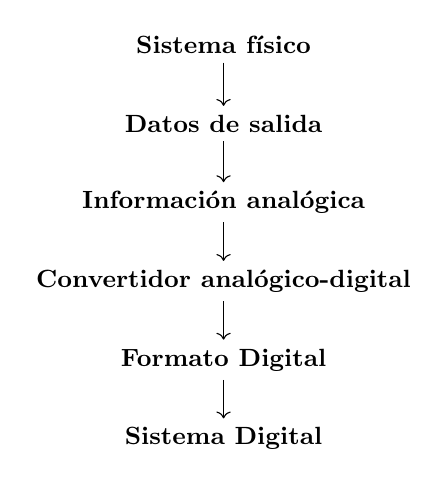
\begin{tikzpicture} 
        \small
        \node (a) at (0, 1) {\textbf{Sistema f\'{i}sico}};
        \node (b) at (0, 0) {\textbf{Datos de salida}};
        \node (c) at (0, -1) {\textbf{Informaci\'{o}n anal\'{o}gica}};
        \node (d) at (0, -2) {\textbf{Convertidor anal\'{o}gico-digital}};
        \node (e) at (0, -3) {\textbf{Formato Digital}};
        \node (f) at (0, -4) {\textbf{Sistema Digital}};

        \draw[->] (a) -- (b);
        \draw[->] (b) -- (c);
        \draw[->] (c) -- (d);
        \draw[->] (d) -- (e);
        \draw[->] (e) -- (f);
    \end{tikzpicture}
\end{center}
\medskip
\normalsize

La ventaja de usar el c\'{o}digo Gray es que la diferencia entre dos n\'{u}meros cualesquiera
es \'{u}nicamente de 1 bit.
\begin{center}
    $(Binario): (0111\,1000)$, $(Gray): (0100\,1100)$
\end{center}

Una aplicaci\'{o}n del c\'{o}digo Gray es en los datos anal\'{o}gicos se representan
mediante el cambio continuo en la posici\'{o}n de un eje.

\subsubsection*{1.7.4 C\'{o}digo ASCII}
El c\'{o}digo ASCII consta de 7-bits para su codificaci\'{o}n, por lo que tiene un conjunto
de 128 combinaciones distintas. Con $b_1 \rightarrow b_7$ siendo $b_7$ el bit m\'{a}s significativo,
por ejemplo: letra A: $100\,0001$, (columna 100, fila 0001).

Contiene 94 caracteres imprimibles y 34 caracteres no imprimibles. Estos no imprimibles son 
caracteres de control.
\begin{itemize}
    \item 26 letras min\'{u}sculas y 26 letras may\'{u}sculas. (52)
    \item 10 d\'{i}gitos decimales. (10)
    \item 32 caracteres especiales. (32)
\end{itemize}
\medbreak

\subsubsection*{1.7.5 Tipos de caracteres de control}

\begin{enumerate}
    \item \textbf{Creadores de Formato}

    Controlan la forma de imprimir, controles conocidos $\rightarrow$ m\'{a}quinas de escribir.
    \begin{itemize}
        \item (BS): Retroceso
        \item (HT): Tabulador Horizontal
        \item (CR): Retorno de carro
    \end{itemize}

    \item \textbf{Separadores de Informaci\'{o}n}

    Separan datos en divisiones como p\'{a}rrafos, l\'{i}neas, p\'{a}ginas, etc.
    \begin{itemize}
        \item (RS): Separador de Registros
        \item (FS): Separador de Archivos
    \end{itemize}

    \item \textbf{Controladores de Informaci\'{o}n}

    Transmisi\'{o}n de datos entre terminales remotas.
    \begin{itemize}
        \item (STX): Inicio de Texto
        \item (ETX): Fin de Texto
    \end{itemize}

    Encuadran un mensaje entre l\'{i}neas telef\'{o}nicas.
\end{enumerate}
(8 bits) $\rightarrow$ (1 byte) $\rightarrow$ (1 car\'{a}cter ASCII), \\
Se almacena 1 Byte por car\'{a}cter ASCII.

\subsubsection*{1.7.6 C\'{o}digo para detectar errores}

Para poder detectar errores en la comunicaci\'{o}n de datos, se agrega un bit extra.
Este bit indica la paridad:

\textbf{(Paridad):} Se refiere a la cantidad de bits 1's en un byte. Si la cantidad de
bits 1's es par, se le asigna un 0, si es impar, se le asigna un 1. Es m\'{a}s com\'{u}n
la paridad par.

\begin{verse}
    El bit de paridad se transmite, \\
    el receptor verifica la paridad del byte recibido, \\
    si la paridad es correcta, se asume que no hay error, \\
    si la paridad es incorrecta, se asume que hay un error.
\end{verse}

\subsection*{1.8 Almacenamiento Binario y Registros}

La informaci\'{o}n binaria $\rightarrow$ debe existir f\'{i}sicamente, \\
medio de almacenamiento en bits $\rightarrow$ registro, \\
un registro de $\rightarrow$ $n$ bits.
\medbreak

El estado de un registro es una tupla de $n$ bits; \\
el contenido $\rightarrow$ funci\'{o}n, la interpretaci\'{o}n $\rightarrow$ informaci\'{o}n.
\medbreak

Un registro de 16 bits:
\begin{center}
    1100001111001001
\end{center} 

Un registro puede:
\begin{itemize}
    \item \begin{center}
        \textbf{Almacenar datos} \\
        elementos discretos de informaci\'{o}n.
    \end{center}
    \item \begin{center}
        \textbf{Almacenar instrucciones} \\
        misma configuraci\'{o}n de bits, distinta interpretaci\'{o}n.
    \end{center}
\end{itemize}
\medbreak

Manipulaci\'{o}n de variables binarias $\rightarrow$ circuitos l\'{o}gicos digitales.
\medbreak
Transferencia de registros $\rightarrow$ operaci\'{o}n b\'{a}sica en sistemas digitales.
\medbreak

\subsection*{1.9 L\'{o}gica Binaria}

\begin{center}
    \textbf{Variables} $\rightarrow$ 2 valores discretos, \\
    \textbf{Operaciones} $\rightarrow$ 3 operaciones l\'{o}gicas.
\end{center}
\medbreak

\begin{flushleft}
    Se habla en t\'{e}rminos de bits, \\
    en valores de (0's y 1's), \'{a}lgebra booleana.
\end{flushleft}
\medbreak

\begin{center}
    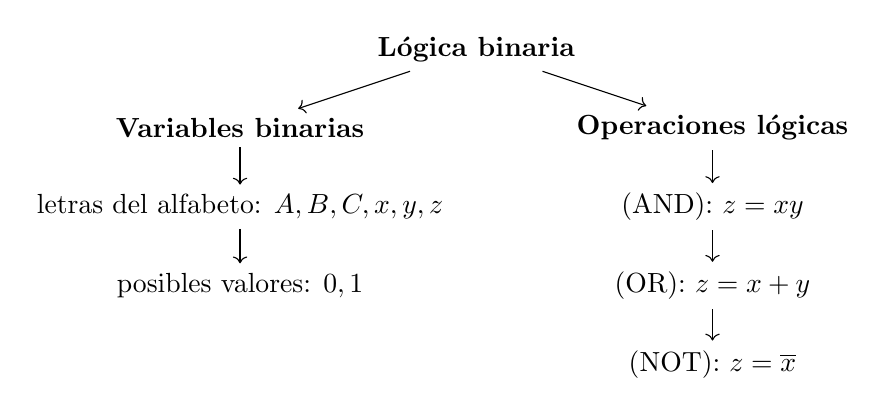
\begin{tikzpicture} 
        \node (a) at (0, 1) {\textbf{L\'{o}gica binaria}};
        \node (b) at (-3, 0) {\textbf{Variables binarias}};
        \node (c) at (3, 0) {\textbf{Operaciones l\'{o}gicas}};
        \node (d) at (-3, -1) {letras del alfabeto: $A, B, C, x, y, z$};
        \node (h) at (-3, -2) {posibles valores: $0, 1$};
        \node (e) at (3, -1) {(AND): $z = xy$};
        \node (f) at (3, -2) {(OR): $z = x + y$};
        \node (g) at (3, -3) {(NOT): $z = \overline{x}$};

        \draw[->] (a) -- (b);
        \draw[->] (a) -- (c);

        \draw[->] (b) -- (d);
        \draw[->] (d) -- (h);

        \draw[->] (c) -- (e);
        \draw[->] (e) -- (f);
        \draw[->] (f) -- (g);
    \end{tikzpicture}
\end{center}

\subsubsection*{1.9.1 Distintas interpretaciones}
\begin{flushleft}
    aritm\'{e}tica binaria: \\
    \begin{center}
        $1 + 1 = 10$
    \end{center}

    l\'{o}gica binaria: \\
    \begin{center}
        $1 + 1 = 1$
    \end{center}
\end{flushleft}

\subsubsection*{1.9.2 Compuertas l\'{o}gicas}
Son dispositivos que operan 1 o m\'{a}s entradas binarias para producir una salida binaria.

\begin{center}
    (AND), (OR), (NOT)
\end{center}

\newpage
\section*{2. \'{A}lgebra booleana y compuertas l\'{o}gicas}
\paragraph*{}
\normalsize

\subsection*{2.1 Definiciones b\'{a}sicas}
En el \'{a}lgebra booleana, al igual que en todos los sitemas matem\'{a}ticos deductivos,
se define con un conjunto de elementos, un conjunto de operadores y varios axiomas.
Un conjunto de elementos es cualquier colecci\'{o}n de objetos con alguna propiedad en 
com\'{u}n. 

\subsubsection*{2.1.1 Conjunto de elementos}
Si $S$ es un conjunto y $x$ y $y$ son ciertos objetos, entonces $x \in S$, se denota que
$x$ es un miembro del conjunto $S$, $S$, y $y \notin S$, denota que $y$ no es un miembro
del conjunto $S$. $A = \{1, 2, 3, 4\}$, denota que estos elementos son miembros del conjunto
$A$. 

\subsubsection*{2.1.2 Conjunto de operadores}
Un operador binario definido sobre un conjunto $S$ de elementos es una regla que asigna a
cada par de elementos de $S$ un elemento \'{u}nico de $S$. Por ejemplo, $a * b = c$.
Se designa $*$ como operador binario si especifica una regla para encontrar $c$ a partir
del par $(a, b)$ y adem\'{a}s si $a, b, c \in S$. Por contraparte no se designa operador
binario si se descubre que $a, b \in S$, pero $c \notin S$.

\subsubsection*{2.1.3 Conjunto de axiomas}
\begin{enumerate}
    \item \textbf{Cerradura}. Un conjunto $S$ es cerrado respecto a un operador binario si, por
    cada par de elementos de $S$, el operador especifica una regla para obtener un elemento
    \'{u}nico de $S$. Por ejemplo, el conjunto de n\'{u}meros naturales $N = \{1, 2, 3,... \}$
    el operador binario m\'{a}s $(+)$. Pero no es cerrado respecto al operador binario menos
    $(-)$, por las reglas de la resta aritm\'{e}tica. 

    \item \textbf{Ley asociativa}. Se dice que un operador binario $*$ sobre un conjunto $S$ es
    asociativo si:
    \begin{center}
        $(x * y) * z = x * (y * z)$ para todos $x, y, z \in S$
    \end{center}

    \item \textbf{Ley conmutativa}. Se dice que un operador binario $*$ sobre un conjunto $S$ es
    conmutativo si
    \begin{center}
        $x * y = y * x$ para todos $x, y \in S$
    \end{center}

    \item \textbf{Elemento identidad}. Se dice que un conjunto $S$ tiene un elemento de identidad
    respecto a una operaci\'{o}n binaria $*$ sobre $S$ si existe un elemento $e \in S$ con la propiedad
    \begin{center}
        $e * x = x * e = x$ para todos $x \in S$
    \end{center} 

    \item \textbf{Inverso}. Se dice que un conjunto $S$, que tiene el elemento de identidad $e$ respecto a
    un operador $*$, tiene un inverso si, para todo $x \in S$, existe un elemento $y \in S$ tal que
    \begin{center}
        $x * y = e$
    \end{center}

    \item \textbf{Ley distributiva}. Si $*$ y $\cdot$ son dos operadores binarios sobre un conjunto $S$, 
    decimos que $*$ es distributivo sobre $\cdot$ si
    \begin{center}
        $x * (y \cdot z) = (x * y) \cdot (x * z)$
    \end{center}
\end{enumerate}

\subsection*{2.2 Definici\'{o}n axiom\'{a}tica del \'{a}lgebra booleana}
En 1854, \textbf{George Boole} introdujo un tratamiento sistem\'{a}tico de la l\'{o}gica. En 1938
\textbf{C. E. Shannon} introdujo un \'{a}lgebra booleana de dos valores tambi\'{e}n llamada \textbf{\'{a}lgebra
de conmutaci\'{o}n}.

Este \'{a}lgebra es una estructura algebraica definida por un conjunto de elementos $B$, junto con dos
operadores binarios, $+$ y $\cdot$, y seis postulados que introdujo \textbf{Huntington}.

\begin{enumerate}
    \item \textbf{Cerradura} \\
    Cerradura respecto al operador $+$. \\
    Cerradura respecto al operador $\cdot$.

    \item \textbf{Elemento identidad} \\
    Elemento identidad con respecto a $+$, designado por 0: $x + 0 = 0 + x = x$. \\
    Elemento identidad con respecto a $\cdot$, designado por 1, $x \cdot 1 = 1 \cdot x = x$.

    \item \textbf{Conmutativa} \\
    Conmutativa respecto a $+$: $x + y = y + x$. \\
    Conmutativa respecto a $x$: $x \cdot y = y \cdot x$.

    \item \textbf{Distributiva} \\
    $\cdot$ es distributivo sobre $+$: $x \cdot (y + z) = (x \cdot y) + (x \cdot z)$. \\ 
    $+$ es distributivo sobre $\cdot$: $x + (y \cdot z) = (x + y) \cdot (x + z)$.  

    \item \textbf{Complemento} \\
    Para cada elemento $x \in B$, existe un elemento un elemento $x' \in B$, tal que 
    $x + x' = 1$ y $x \cdot x' = 0$.

    \item \textbf{Dualidad} \\
    Existen al menos dos elementos $x, y \in B$, tales que $x \neq y$. 
\end{enumerate}

\newpage
\subsection*{2.3 Funciones booleanas}
El \'{a}lgebra booleana se ocupa de variables binarias y operaciones l\'{o}gicas. Una
funci\'{o}n booleana, es descrita por una expresi\'{o}n algebraica que consta de variables
binarias, contantes 0 y 1, y s\'{i}mbolos l\'{o}gicos de operaci\'{o}n. Por ejemplo:
\begin{center}
    $F_1 = x + y'z$
\end{center}

La funci\'{o}n $F_1$ es igual a 1 si $x$ es igual a 1 o si tanto $y'$ como z son iguales a 1.
En los dem\'{a}s casos, $F_1$ es igual a 0.

Se puede representar una funci\'{o}n booleana en una \textbf{tabla de verdad}. Una tabla de verdad
es una lista de \textit{combinaciones} de unos y ceros asignados a las variables binarias y una
columna que muestra el valor de la funci\'{o}n para cada combinaci\'{o}n. El n\'{u}mero de filas
de la tabla es de $2^n$, donde $n$ es el n\'{u}mero de variables de la funci\'{o}n. Contando de
0 hasta $2^n - 1$.

\begin{table}[h]
    \centering
    \begin{tabular}{ccc|c}
        \toprule
        $x$ & $y$ & $z$ & $F_1$ \\
        \midrule
        0 & 0 & 0 & 0 \\
        0 & 0 & 1 & 1 \\
        0 & 1 & 0 & 0 \\
        0 & 1 & 1 & 0 \\
        1 & 0 & 0 & 1 \\
        1 & 0 & 1 & 1 \\
        1 & 1 & 0 & 1 \\
        1 & 1 & 1 & 1 \\
        \bottomrule
    \end{tabular}
    \caption{Tabla de verdad de $F_1 = x + y'z$}
    \label{tab:truth_table}
\end{table}
\medbreak

\begin{figure}[!ht]
    \centering
    \begin{circuitikz}
        \draw (10, 1) node[american or port, scale=0.8] (or) {};
        \draw (0, 1.15) node[left] {$x$} -- (or.in 1);
        \draw (or.out) -- (10.5, 1) node[right] {$F_1$};
        
        \draw (7, -0.5) node[american and port, scale=0.8] (and) {};
        \draw (7, -0.5) node[right] {} -| ++(1, 1) |- (or.in 2);
        \draw (0, -0.76) node[left] {$z$} -- (and.in 2);
        
        \draw (4, -0.29) node[american not port, scale=0.4] (not) {};
        \draw (4.2, -0.29) node[right] {} -- (and.in 1);
        \draw (0, -0.29) node[left] {$y$} -- (not.in);
    \end{circuitikz}
    \caption{Circuito l\'{o}gico de $F_1 = x + y'z$}
\end{figure}
\medbreak

Una funci\'{o}n booleana se puede transformar de una expresi\'{o}n algebraica a un diagrama
de circuitos hecho con compuertas l\'{o}gicas. Solo hay una forma de representar una funci\'{o}n
booleana en una tabla de verdad. Sin embargo, la funci\'{o}n en forma algebraica, puede expresarse
de varias maneras. Manipulando una expresi\'{o}n booleana se puede obtener una expresi\'{o}n m\'{a}s
simple de la misma funci\'{o}n y as\'{i} reducir el n\'{u}mero de compuertas l\'{o}gicas del circuito.

\newpage
Consideremos ahora esta funci\'{o}n booleana y su posible simplificaci\'{o}n:
\begin{align*}
    F_2 &= x'y'z + x'yz + xy' + xy' \\
    &= x'z(y' + y) \\
    &= x'z + xy'
\end{align*}

La funci\'{o}n de tres terminos y ocho literales se reduce a \'{u}nicamente dos t\'{e}rminos 
y cuatro literales. Ambas realizan la misma funci\'{o}n, pero es preferible la forma simplificada
porque requiere menos compuertas l\'{o}gicas.

\subsubsection*{2.3.1 Manipulaci\'{o}n algebraica}
Se define una literal como una sola variable dentro de un t\'{e}rmino. Si se reduce el n\'{u}mero
de t\'{e}rminos, el n\'{u}mero de literales, o ambas, en una expresi\'{o}n booleana, podr\'{i}a 
obtenerse un circuito m\'{a}s simple. Las funciones de hasta cinco variables se pueden simplificar
con el m\'{e}todo del mapa. Se describir\'{a} m\'{a}s adelante.

\subsubsection*{2.3.2 Complemento de una funci\'{o}n}
El complemento de una funci\'{o}n $F$ es $F'$, se obtiene intercambiando los ceros por unos y unos 
por ceros en el valor de $F$. Esto se puede deducir algebraicamente usando el teorema de 
\textbf{DeMorgan}. Adem\'{a}s este se puede extender a tres o m\'{a}s variables. As\'{i}:
\begin{align*}
    (A + B + C)' &= (A + x)' \\
    &= A'x' \\
    &= A'(B + C)' \\
    &= A'(B'C') \\
    &= A'B'C'
\end{align*}
\medbreak

El teorema de DeMorgan se puede generalizar de la siguiente manera:
\begin{center}
    $(A + B + C + D + ... + F)' = A'B'C'D'...F'$ \\
    $(ABCD...F)' = A' + B' + C' + D' + ... + F'$
\end{center}

Otro procedimiento m\'{a}s sencillo para obtener el complemento de una funci\'{o}n consiste
en obtener el dual de la funci\'{o}n y complementar cada literal. Esto es en consecuencia del
teorema de DeMorgan. El dual de una funci\'{o}n se obtiene intercambiando los operadores \textbf{AND}
y \textbf{OR}, y unos y ceros. Ejemplo:
\begin{flushleft}
    $F_1 = x'yz' + x'y'z$ \\
    El dual de $F_1$ es $(x' + y + z')(x' + y' + z)$ \\
    Complementando cada literal: $(x + y' + z)(x + y + z') = F_1'$ 
\end{flushleft}
\newpage

\subsection*{2.4 Formas can\'{o}nicas y est\'{a}ndar}
\begin{table}[h]
    \centering
    \begin{tabular}{ccccccc}
        \toprule
        &  &  & \multicolumn{2}{c}{\textbf{Minit\'{e}rminos}} & \multicolumn{2}{c}{\textbf{Maxit\'{e}rminos}} \\
        \cmidrule{4-5} \cmidrule{6-7}
        $x$ & $y$ & $z$ & T\'{e}rminos & Designaci\'{o}n & T\'{e}rminos & Designaci\'{o}n \\
        \midrule
        0 & 0 & 0 & $x'y'z'$ & $m_0$ & $x + y + z$ & $M_0$ \\
        0 & 0 & 1 & $x'y'z$ & $m_1$ & $x + y + z'$ & $M_1$ \\
        0 & 1 & 0 & $x'yz'$ & $m_2$ & $x + y' + z$ & $M_2$ \\
        0 & 1 & 1 & $x'yz$ & $m_3$ & $x + y' + z'$ & $M_3$ \\
        1 & 0 & 0 & $xy'z'$ & $m_4$ & $x' + y + z$ & $M_4$ \\
        1 & 0 & 1 & $xy'z$ & $m_5$ & $x' + y + z'$ & $M_5$ \\
        1 & 1 & 0 & $xyz'$ & $m_6$ & $x' + y' + z$ & $M_6$ \\
        1 & 1 & 1 & $xyz$ & $m_7$ & $x' + y' + z'$ & $M_7$ \\
        \bottomrule
    \end{tabular}
    \caption{Minit\'{e}rminos y maxit\'{e}rminos para tres variables binarias} 
    \label{tab:miniterminos_maxiterminos} 
\end{table}

Una variable binaria podr\'{i}a aparecer en su forma normal ($x$) o en su forma complementada
($x'$). Ahora si se considerada dos variables binarias $x$ y $y$ que se combinan con una operaci\'{o}n
AND. Se pueden obtener cuatro combinaciones posibles: $x'y'$, $x'y$, $xy'$ y $xy$. Cada uno de
estos cuatro t\'{e}rminos AND es un \textit{minit\'{e}rmino, o producto est\'{a}ndar}. De igual
manera se puede combinar $n$ variables para formar $2^n$ minit\'{e}rminos. Se enumeran del 0 a $2^n - 1$. 
Cada minit\'{e}rmino se obtiene de un t\'{e}rmino AND de las n variables, se designa un s\'{i}mbolo $m_j$,
donde $j$ denota el equivalente decimal del n\'{u}mero binario que representa el minit\'{e}rmino.

Asimismo, $n$ variables que forman un t\'{e}rmino OR, llamado \textit{maxit\'{e}rmino o suma est\'{a}ndar}.
Cabe decir que cada maxit\'{e}rmino es el complemento de su minit\'{e}rmino correspondiente y viceversa.
As\'{i}, expresar las combinaciones 001, 100 y 111 como $x'y'z'$, $xy'z'$ y $xyz$, respectivamente. Puesto 
que cada uno de estos minit\'{e}rminos hace que $f_1 = 1$, se tiene:
\begin{center}
    $f_1 = x'y'z + xy'z' + xyz = m_1 + m_4 + m_7$ 
\end{center}

\subsubsection*{2.4.1 Forma can\'{o}nica: suma de minit\'{e}rminos}
\begin{flushleft}
    Esto ilustra una propiedad importante del \'{a}lgebra booleana: cualquier funci\'{o}n booleana se puede
    expresar como \textit{una suma de minit\'{e}rminos}. Ahora podemos hacer lo mismo pero con maxit\'{e}rminos,
    de modo qu\'{e} el complemento de $f_2$ se lee:
\end{flushleft}
\begin{center}
    $f_2' = x'y'z' +x'yz' + x'yz + xy'z + xyz'$    
\end{center}

Ejemplo de suma de minit\'{e}rminos:
\begin{flushleft}
    Expresar la funci\'{o}n booleana $F = A + B'C$ como la suma de minit\'{e}rminos. Por lo tanto:
    \begin{center}
        $A = A(B + B') = AB + AB'$
    \end{center}
    A\'{u}n le falta una variable:
    \begin{align*}
        A &= AB(C + C') + AB'(C + C') \\
        &= ABC + ABC' + AB'C + AB'C' \\
    \end{align*}
    Al segundo t\'{e}rmino, B'C , le falta una variable:
    \begin{center}
        $B'C = B'C(A + A') = AB'C + A'B'C$
    \end{center}
    Al combinar todo se tiene:
    \begin{align*}
        F &= A + B'C \\
        &= ABC + ABC' + AB'C + AB'C' + AB'C + A'B'C \\
    \end{align*}
    Como AB'C aparece dos veces, se puede simplificar:
    \begin{align*}
        F &= ABC + ABC' + AB'C + AB'C' + A'B'C \\
        &= A'B'C + AB'C' + AB'C + ABC' + ABC \\ 
        &= m_1 + m_4 + m_5 + m_6 + m_7
    \end{align*}
\end{flushleft}

En ocasiones conviene expresar la funci\'{o}n booleana, de la siguiente notaci\'{o}n:
\begin{center}
    $F(A, B, C) = \sum(1, 4, 5, 6, 7)$
\end{center}

\subsubsection*{2.4.2 Forma can\'{o}nica: producto de maxit\'{e}rminos}
\begin{flushleft}
    Si obtenemos el complemento de $f_2'$, se obtiene $f_2$:
\end{flushleft}
\begin{align*}
    f_2 &= (x + y + z)(x + y' + z)(x + y' + z')(x' + y + z')(x' + y' + z) \\
    &= M_0 \cdot M_2 \cdot M_3 \cdot M_5 \cdot M_6
\end{align*}

Este ejemplo ilusta la segunda propiedad del \'{a}lgebra booleana, cualquier funci\'{o}n booleana se puede
expresar como un \textit{producto de maxit\'{e}rminos}. Se dice que las funciones booleanas 
expresadas como suma de minit\'{e}rminos o producto de maxit\'{e}rminos est\'{a}n en \textbf{forma can\'{o}nica}.
\medbreak

Ejemplo de producto de maxit\'{e}rminos:
\begin{flushleft}
    Expresar la funci\'{o}n booleana $F = xy + x'z$ en forma de producto de maxit\'{e}rminos. Por lo tanto:
    \begin{align*}
        F &= xy + x'z = (xy + x')(xy + z) \\
        &= (x + x')(y + x')(x + z)(y + z) \\
        &= (x' + y)(x + z)(y + z)
    \end{align*}
    La funci\'{o}n tiene tres variables, $x$, $y$ y $z$. A cada t\'{e}rmino OR le falta una variable; por tanto:
    \begin{center}
        $x' + y = x' + y + zz' = (x' + y + z)(x' + y + z')$ \\
        $x + z = x + z + yy' = (x + y + z)(x + y' + z)$ \\
        $y + z = y + z + xx' = (x + y + z)(x' + y + z)$
    \end{center}
    Despu\'{e}s de combinar todos los t\'{e}rminos y eliminar los que se repiten; se tiene:
    \begin{align*}
        F &= (x + y + z)(x + y' + z)(x' + y + z)(x' + y + z') \\
        &= M_0 \cdot M_2 \cdot M_4 \cdot M_5
    \end{align*}
    Una forma c\'{o}moda de expresar esta funci\'{o}n es:
    \begin{center}
        $F(x, y, z) = \prod(0, 2, 4, 5)$
    \end{center}
\end{flushleft}

\subsection*{2.5 Conversi\'{o}n entre formas can\'{o}nicas}
El complemento de una funci\'{o}n expresado como la suma de minit\'{e}rminos es igual a la suma
de los minit\'{e}minos que faltan en la funci\'{o}n original. Por ejemplo:

\begin{center}
    $F(A, B, C) = \sum(1, 4, 5, 6, 7)$
\end{center}
\begin{flushleft}
    Su complemento se expresa como
\end{flushleft}
\begin{center}
    $F'(A, B, C) = \sum(0, 2, 3) = m_0 + m_2 + m_3$
\end{center}

\begin{flushleft}
    Ahora si determinamos el complemento de $F'$, se obtiene $F$:
\end{flushleft}
\begin{center}
    $F = (m_0 + m_2 + m_3)' = m_0' \cdot m_2' \cdot m_3' = M_0M_2M_3 = \prod(0, 2, 3)$
\end{center}

Por lo que se puede ver la relaci\'{o}n entre minit\'{e}rminos y maxim\'{i}nimos:
\begin{center}
    $m_j' = M_j$
\end{center}
Th

Este ejemplo ilustra la conversi\'{o}n de una funci\'{o}n expresada como la suma de minit\'{e}rminos
y su equivalente como el producto de maxit\'{e}rminos.

Si tenemos:
\begin{center}
    $F = xy + x'z$
\end{center}

\begin{flushleft}
    La suma de minit\'{e}rminos:
\end{flushleft}
\begin{center}
    $F(x, y, z) = \sum(1, 3, 6, 7)$
\end{center}
\begin{flushleft}
    El producto de maxit\'{e}rminos:
\end{flushleft}
\begin{center}
    $F(x, y, z) = \prod(0, 2, 4, 5)$
\end{center}
\newpage

\subsection*{2.6 Formas est\'{a}ndar}
Las formas can\'{o}nicas son formas b\'{a}sicas al leer una funci\'{o}n de su tabla de verdad,
pero casi nunca son las que tienen el n\'{u}mero m\'{i}nimo de literales, porque cada minit\'{e}rmino
o maxit\'{e}rmino debe contener, por definici\'{o}n, todas las variables, complementadas o sin complementar.

Otra manera de expresar las funciones booleanas es en forma est\'{a}ndar. Existen dos tipos de forma est\'{a}ndar:
\textit{la suma de productos y el producto de sumas}. La suma de productos contiene t\'{e}rminos AND, llamados
\textit{t\'{e}rminos de producto}, ejemplo:
\begin{center}
    $F_1 = y' + xy + x'yz'$
\end{center}
Por lo consecuente se puede crear un circuito con una implementaci\'{o}n de dos niveles. El producto de sumas contiene
t\'{e}rminos OR, llamados \textit{t\'{e}rminos de suma}, ejemplo:
\begin{center}
    $F_2 = x(y' + z)(x' + y + z)$
\end{center}
El tipo est\'{a}ndar produce una estructura de compuertas de dos niveles.

\subsection*{2.7 Otras operaciones l\'{o}gicas}
Hay $2^2n$ funciones para n variables binarias, en el caso de dos variables $n = 2$, existe 16 posibles funciones booleanas.

\begin{table}[h]
    \centering
    \begin{tabular}{cccc}
        \toprule
        Funciones booleanas & S\'{i}mbolo operador & Nombre & Comentarios \\ 
        \midrule
        $F_0 = 0$ & & Nula & Constante binaria 0 \\
        $F_1 = xy$ & $x \cdot y$ & AND &$x$ y $y$ \\ 
        $F_2 = xy'$ & $x/y$ & Inhibici\'{o}n & x, pero no y \\
        $F_3 = x$ & & Transferencia & $x$ \\
        $F_4 = x'y$ & $y/x$ & Inhibici\'{o}n & y, pero no x \\
        $F_5 = y$ & & Transferencia & $y$ \\
        $F_6 = xy' + xy$ & $x \oplus y$ & OR exclusivo & $x$ o $y$, pero no ambos \\
        $F_7 = x + y$ & $x + y$ & OR & $x$ o $y$ \\
        $F_8 = (x + y)'$ & $x \downarrow y$ & NOR & No OR \\
        $F_9 = xy + x'y'$ & $(x \oplus y)'$ & Equivalencia & $x$ es igual a $y$ \\
        $F_{10} = y'$ & $y'$ & Complemento & No $y$ \\
        $F_{11} = x + y'$ & $x \subset y$ & Implicaci\'{o}n & Si y, entonces x \\
        $F_{12} = x'$ & $x'$ & Complemento & No $x$ \\
        $F_{13} = x' + y$ & $x \supset y$ & Implicaci\'{o}n & Si x, entonces y \\
        $F_{14} = (xy)'$ & $x \cdot y$ & NAND & No AND \\
        $F_{15} = 1$ & & Identidad & Contante binaria 1 \\
        \bottomrule
    \end{tabular}
\end{table}

\end{document}